% Copyright 2004 by Till Tantau <tantau@users.sourceforge.net>.
%
% In principle, this file can be redistributed and/or modified under
% the terms of the GNU Public License, version 2.
%
% However, this file is supposed to be a template to be modified
% for your own needs. For this reason, if you use this file as a
% template and not specifically distribute it as part of a another
% package/program, I grant the extra permission to freely copy and
% modify this file as you see fit and even to delete this copyright
% notice. 

\documentclass{beamer}
\usepackage{graphicx}
\usepackage{breqn}
\graphicspath{ {images/} }
\usepackage{amsmath}
\usepackage{dsfont}
% There are many different themes available for Beamer. A comprehensive
% list with examples is given here:
% http://deic.uab.es/~iblanes/beamer_gallery/index_by_theme.html
% You can uncomment the themes below if you would like to use a different
% one:
%\usetheme{AnnArbor}
%\usetheme{Antibes}
%\usetheme{Bergen}
%\usetheme{Berkeley}
\usetheme{Berlin}
%\usetheme{Boadilla}
%\usetheme{boxes}
%\usetheme{CambridgeUS}
%\usetheme{Copenhagen}
%\usetheme{Darmstadt}
%\usetheme{default}
%\usetheme{Frankfurt}
%\usetheme{Goettingen}
%\usetheme{Hannover}
%\usetheme{Ilmenau}
%\usetheme{JuanLesPins}
%\usetheme{Luebeck}
%\usetheme{Madrid}
%\usetheme{Malmoe}
%\usetheme{Marburg}
%\usetheme{Montpellier}
%\usetheme{PaloAlto}
%\usetheme{Pittsburgh}
%\usetheme{Rochester}
%\usetheme{Singapore}
%\usetheme{Szeged}
%\usetheme{Warsaw}

\title{Effects of Unemployment Benefits and Uncertainty in Heterogeneous Models}

% A subtitle is optional and this may be deleted
\subtitle{}

\author{Eric, Yannic and Andrian}
% - Give the names in the same order as the appear in the paper.
% - Use the \inst{?} command only if the authors have different
%   affiliation.

%\institute[Universities of Somewhere and Elsewhere] % (optional, but mostly needed)
%{
% \inst{1}%
%  Department of Computer Science\\
%  University of Somewhere
%  \and
%  \inst{2}%
%  Department of Theoretical Philosophy\\
%  University of Elsewhere}
% - Use the \inst command only if there are several affiliations.
% - Keep it simple, no one is interested in your street address.

%\date{Conference Name, 2013}
% - Either use conference name or its abbreviation.
% - Not really informative to the audience, more for people (including
%   yourself) who are reading the slides online

%\subject{Theoretical Computer Science}
% This is only inserted into the PDF information catalog. Can be left
% out. 

% If you have a file called "university-logo-filename.xxx", where xxx
% is a graphic format that can be processed by latex or pdflatex,
% resp., then you can add a logo as follows:

% \pgfdeclareimage[height=0.5cm]{university-logo}{university-logo-filename}
% \logo{\pgfuseimage{university-logo}}

% Delete this, if you do not want the table of contents to pop up at
% the beginning of each subsection:
\AtBeginSubsection[]
{
  \begin{frame}<beamer>{Outline}
    \tableofcontents[currentsection,currentsubsection]
  \end{frame}
}


% Let's get started
\begin{document}



\begin{frame}
  \titlepage
\end{frame}

\begin{frame}{Outline}
  \tableofcontents
  % You might wish to add the option [pausesections]
\end{frame}

% Section and subsections will appear in the presentation overview
% and table of contents.
\section{Part I}
\subsection{}
\begin{frame}{Introduction}
  \begin{itemize}

  \item {1.}
  \end{itemize}
\end{frame}
\section{Part II}
\subsection{}
\begin{frame}{Welfare Measurement}
  \begin{itemize}
  \item {
  Which variable should we look at if we want to say consumers are better off? Output? Consumption?
  }
  \item {
  We want to measure somehow whether consumer welfare increased or not.
  }
  \item {
  But how to measure welfare? Can we compare the utility levels of consumers? And whose utility should we compare in a heterogeneous agent framework?
  }
  \end{itemize}
\end{frame}

\begin{frame}{Life-time Utility}
  \begin{itemize}
  \item {
  We calculate the life-time utility of each agent when the economy is in steady state. One time before the policy change and once after the policy change.
  }
  \item {
  Cannot compare two steady states directly. We need to take the transition into account.
  }
  \item {
  Calculating the exact transition path is troublesome. We follow the approximation by Krussel, Mukoyama, and Sahin (2010) which takes care of the idiosyncratic transition.
  }
  	\begin{itemize}
  	\item {
  	Just place the agents in the first economy with their current assets into the second economy.
  	}
  	\end{itemize}
  \end{itemize}
\end{frame}

\begin{frame}{Welfare Analysis}
  \begin{itemize}
  \item {
  Now we can compare the utility level of the same agent before and after the policy change.
  }
  \item {
  Need to come up with a way to quantify the utility differences sensibly.
  }
  \item {
  We calculate a consumption and a cash equivalent of the policy change.
  }
  \end{itemize}
\end{frame}

\begin{frame}{Consumption Equivalent}
  \begin{itemize}

  \item {
  Permanent change of consumption by factor $\Delta$ that increases life-time
  utility by same amount as policy change:
  }
  \end{itemize}
  \begin{equation}
  U^{2}(e,k) = \mathbb{E}\sum_{t=0}^{\infty}\beta^{t}\frac{(c^{1}_{i,t}\Delta)^{1-\sigma}-1}{1-\sigma}\nonumber
  \end{equation}
  \begin{itemize}
  \item {
  If $ \Delta>1 $ agents prefer policy change $ (U^{2}) $, otherwise they do not want it.
  }
  \end{itemize}
\end{frame}

\begin{frame}{Consumption Equivalent}
  \centering{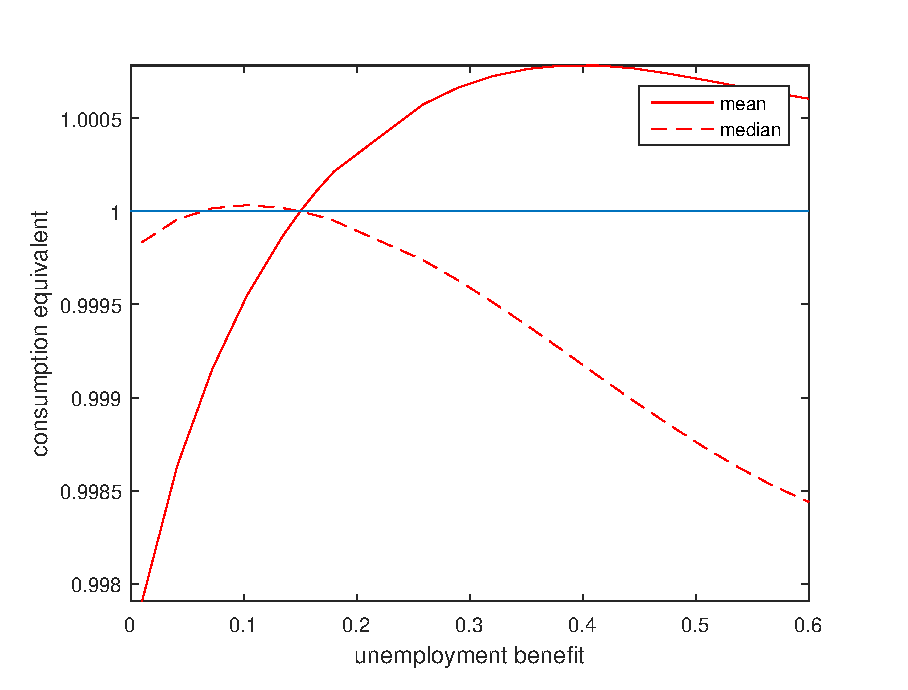
\includegraphics[scale=0.6]{cons_equiv}}
\end{frame}

\begin{frame}{Consumption Equivalent}
  \centering{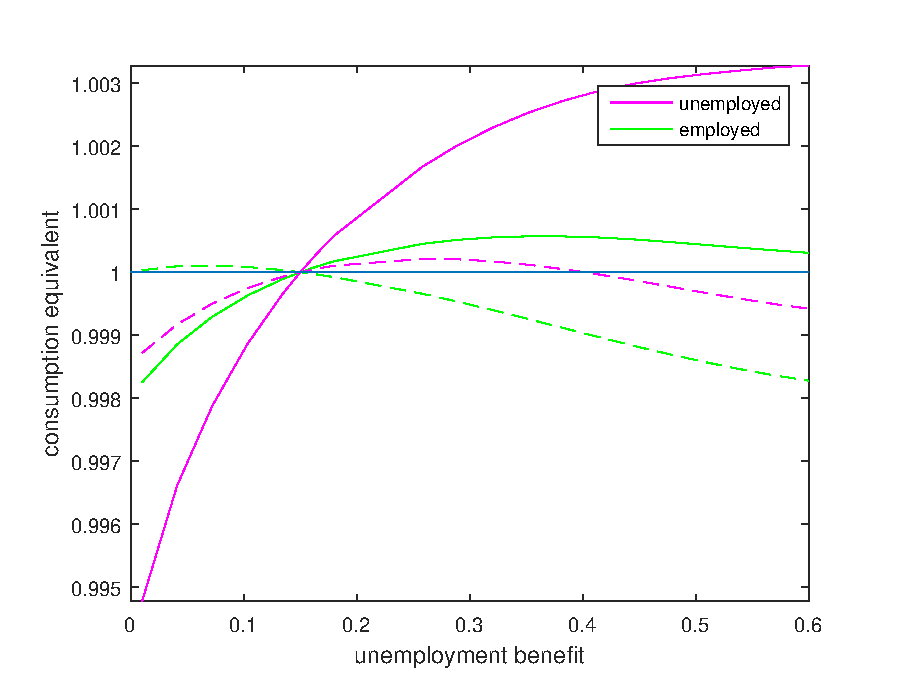
\includegraphics[scale=0.6]{cons_equiv_unemp_emp}}
\end{frame}

\begin{frame}{Consumption Equivalent}
  \begin{itemize}
  \item {
  Summary consumption equivalent
  }
  \item {
  2
  }
  \item {
  3
  }
  \end{itemize}
\end{frame}

\begin{frame}{Cash Equivalent}
  \begin{itemize}
  \item {
  Transfer of $\Delta$ units of wealth in the first period
  }
  \end{itemize}
  
  \begin{equation}
  U^{2}(e,k) = U^{1}(e,k+\Delta) \nonumber
  \end{equation}
  
  \begin{itemize}
  \item {
  If $ \Delta>0 $ agents prefer the policy change $ (U^{2}) $, otherwise not.
  }
  \end{itemize}
\end{frame}

\begin{frame}{Cash Equivalent}
  \centering{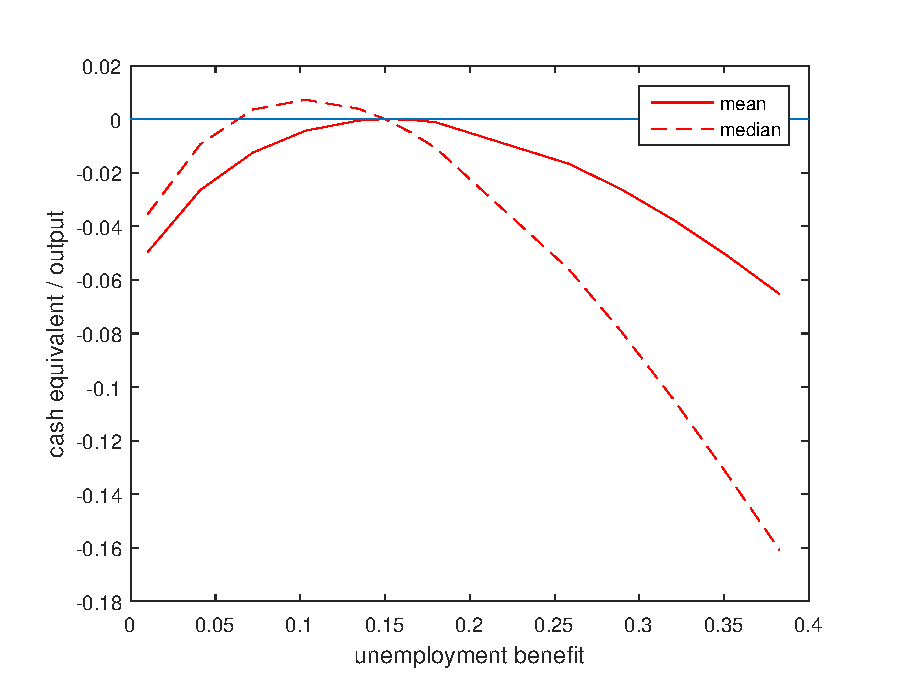
\includegraphics[scale=0.6]{cash_equiv}}
\end{frame}

\begin{frame}{Cash Equivalent}
  \centering{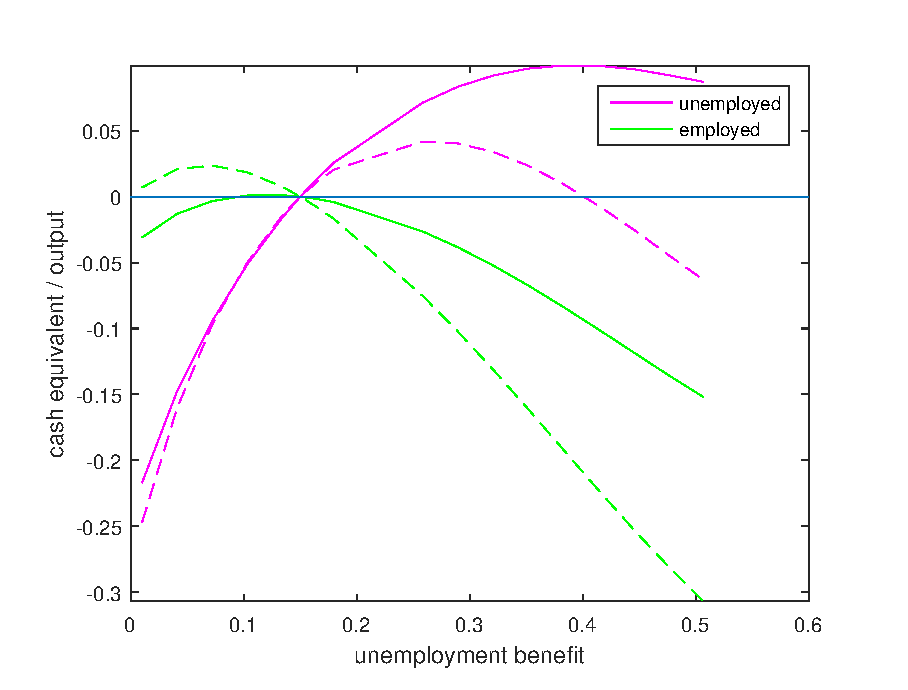
\includegraphics[scale=0.6]{cash_equiv_unemp_emp}}
\end{frame}

\begin{frame}{Cash Equivalent}
  \begin{itemize}
  \item {
  Summary cash equivalent
  }
  \item {
  2
  }
  \item {
  3
  }
  \end{itemize}
\end{frame}

\begin{frame}{Cash vs. Consumption Equivalent}
\centering{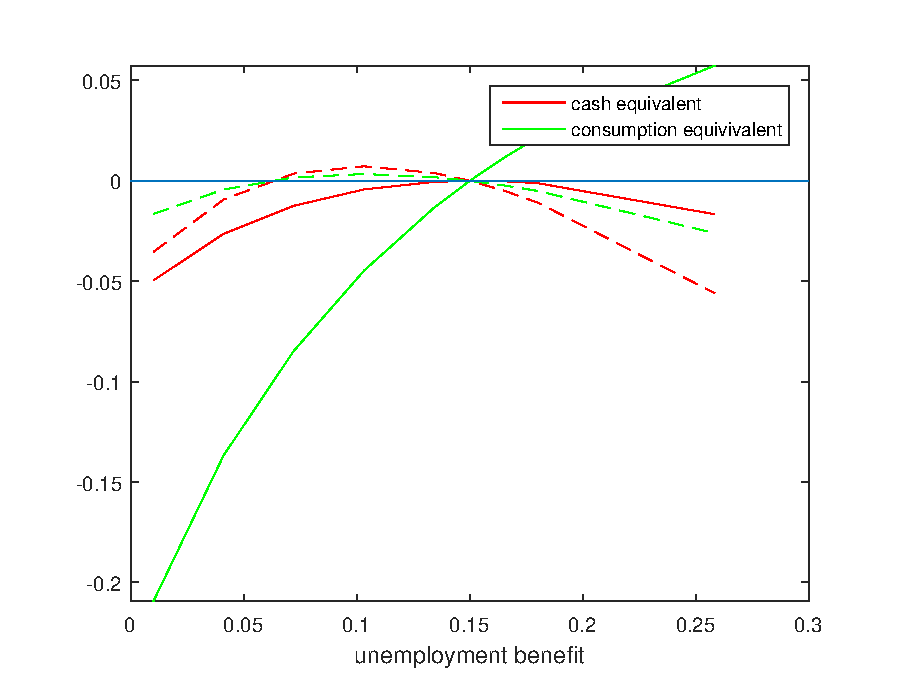
\includegraphics[scale=0.6]{cash_cons_equiv}}
\end{frame}

\begin{frame}{Cash vs. Consumption Equivalent}
  \begin{itemize}
  \item {
  Summary cash vs. consumption equivalent and connection to Andrians part.
  }
  \item {
  2
  }
  \item {
  3
  }
  \end{itemize}
\end{frame}

\section{Part III}
\subsection{}

\end{document}